%%%%%%%%%%%%%%%%%%%%%%%%%%%%%%%%%%%%%%%%
\begin{figure}[thb]
\centering
\begin{subfigure}[b]{0.45\linewidth}
\centering
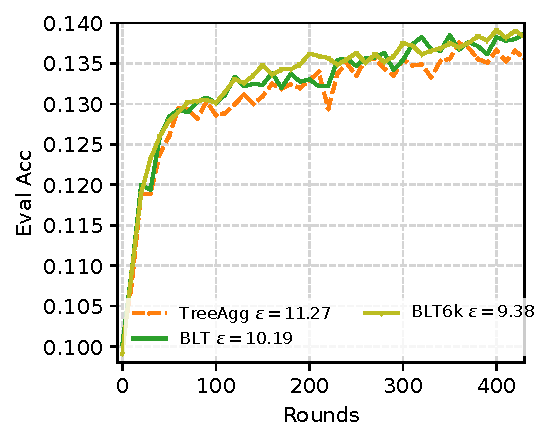
\includegraphics[width=\textwidth]{images/ptpt_acc.pdf}
\caption{\small NWP \ifthenelse{\boolean{acl}}{}{evaluation} accuracy}
\label{fig:example_acc}
\end{subfigure}
%
\begin{subfigure}[b]{0.44\linewidth}
\centering
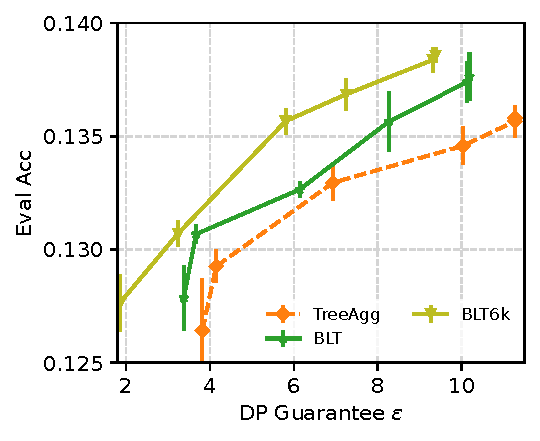
\includegraphics[width=\textwidth]{images/ptpt_priv.pdf}
\caption{\small Privacy-utility trade-off}
\label{fig:example_priv}
\end{subfigure}
%
\ifthenelse{\boolean{acl}}{
\caption{\small NWP evaluation accuracy and the dervied privacy-utility trade-off curves for training the Portuguese LM in Portugal (pt-PT) with DP-FTRL in a FL system. Additional curves for es-ES, id-ID, and pt-BR are provided in \cref{fig:acc_curve,fig:acc_curve2,fig:priv_curve}. \blts achieve better privacy-utility trade-off.}
}{
\caption{\small NWP evaluation accuracy and privacy-utility trade-off curves for training the production Portuguese LM in Portugal (pt-PT) with DP-FTRL in a FL system. Additional curves for es-ES, id-ID, and pt-BR are provided in \cref{fig:acc_curve,fig:priv_curve}, with NWP accuracy zoomed-in for later stage of training in \cref{fig:acc_curve2}. The privacy-utility trade-off curves are derived from NWP accuracy curves: for each selected round $r$, we compute the mean and standard deviation (shown as vertical bars) for accuracy from the rounds in the range of $r\pm10$, and accounting the DP guarantees. \blts achieve better privacy-utility trade-off.}
}\label{fig:example_curve}
\vspace{-0.4cm}
\end{figure}
%%%%%%%%%%%%%%%%%%%%%%%%%%%%%%%%%%%%%%%%